\documentclass[12pt]{article}

\usepackage[utf8]{inputenc}
\usepackage{amsmath}
\usepackage{fancyhdr}
\usepackage{graphicx}
\usepackage{vmargin}
\usepackage{chemfig}
\usepackage{tikz}
\usepackage{pgfplots}

%%%%%%%%%%%%%%%%%%%%%%%%%%%%%%%%%%%%%%%%%%%%%%%%%%%%%%%%%%%%%%%%%%%%%%%%%%

\setmarginsrb{3 cm}{2.5 cm}{3 cm}{2.5 cm}{1 cm}{1.5 cm}{1 cm}{1.5 cm}
\pagestyle{fancy}
\fancyhf{}
\rhead{Jeppe Møldrup}
\chead{Studieretnings Opgave}
\lhead{22/06-2018}
\rfoot{side \thepage}
\renewcommand{\contentsname}{Indholdsfortegnelse}
\renewcommand{\baselinestretch}{1.5}

%%%%%%%%%%%%%%%%%%%%%%%%%%%%%%%%%%%%%%%%%%%%%%%%%%%%%%%%%%%%%%%%%%%%%%%%%%

\begin{document}

\begin{abstract}
Abstract
\end{abstract}
\pagebreak

\tableofcontents
\pagebreak

\section{Indledning}
Indledning
\section{Redegørelse}
Differenskvotient er sekantens hældning af to punkter $x_{0}$ og $x_{0}+\Delta x$ på en differentiabel graf.
Differentialkvotient er så tangentens hældning af et punkt $x_{0}$ på en differentiabel graf.\\
Se bilag 1.\\
Hastighed er den udledte funktion fra en stedfunktion dvs. en graf for tid og strækning, hvor den udledte funktion er en graf for tid og strækning per tid. Så hastighed er ændringen af hastighed per tid og har enheden $\frac{m}{s}$.
Acceleration er så den udledte funktion fra en hastighedsfunktion. Dvs. at acceleration er ændringen af hastighed per tid og har enheden $\frac{m}{s^2}$.\\
Teorien bag luftmodstand er at jo større tværsnitsarealet eller frontarealet for et legeme er og jo hurtigere legemet bevæger sig gennem luften, desto større er den luftmodstand der virker på legemet. Luftmodstanden vil være en kraft der peger den anden retning end den retning som legemet bevæger sig,
fordi legemet skubber luften i den retning legemet bevæger sig og så ifølge newtons tredje lov bliver legemet så udsat for en kraft der er lige så stor men omvendt af den legemet udsætter luften for.


\section{Forsøg med kageform}
Formålet med forsøget er at finde en sammenhæng mellem faldhastighed af et legeme og luftmodstanden. Forsøget går så ud på at vi lader nogle papir muffinforme falde gennem luften
hvor vi så måler papirformene med en bevægelsesføler. For at få noget variation ændrer vi på massen af papirformene ved at stakke flere papirforme oveni hinanden og lade dem falde sammen.\\
Teorien bag det er at kageformene bliver udsat for 2 kræfter. Tyngdekraften og luftmodstanden. Og når kageformene så når et punkt hvor de falder med konstant hastighed, ved vi fra newtons 1. lov
at summen af alle kræfter er lig 0. Og da luftmodstanden i dette tilfælde laver en kraft der er omvendt af tyngdekraften ved vi at de to krafter må være lig med hinanden hvir kageformen falder med
en konstant hastighed.

\subsection{Ligning for $F_{luft}$}
For at finde en ligning for $F_{luft}$ starter vi med at måle en hel masse data
med kageformene. Her finder vi så et område i vores data hvor vi kan se at kageformen
falder med konstant hastighed. De kan vi se fordi stedfunktionen er lineær og derfor er
den udledte funktion konstant. Så skriver vi så dataet ned i tabellen nedenunder
\begin{center}
  \begin{tabular}{| c | c | c | c | c | c | c | c | c |}
        \hline
        $v(\frac{m}{s})$ & $0.981$ & $1.14$ & $1.67$ & $2.59$ & $1.65$ & $3.05$ & $1.89$ & $1.99$ \\
        \hline
        $m(g)$ & $6.91$ & $14.07$ & $34.83$ & $62.04$ & $23.97$ & $69.51$ & $28.68$ & $40.47$ \\
        \hline
  \end{tabular}
\end{center}

Som jeg forklarede i redegørelsen for forsøget ved vi at når hastigheden er konstant. Og det kun er tyngdekraften og luftmodstanden der virker på kageformen
så vil tyngdekraften og luftmodstanden være lige store. Så vi bruger formlen
$$F_{t}=m \cdot a$$
Til at finde størrelsen på tyngdekraften der virker på kageformen. \\
Og da $F_{t}=F_{luft}$(Vi kigger kun på størrelsen af kraften her, da det er den der er ens)
kan vi bare indsætte værdierne in i tabellen nedenunder
\begin{center}
  \begin{tabular}{| c | c | c | c | c | c | c | c | c |}
        \hline
        $v(\frac{m}{s})$ & $0.981$ & $1.14$ & $1.67$ & $2.59$ & $1.65$ & $3.05$ & $1.89$ & $1.99$ \\
        \hline
        $m(g)$ & $6.91$ & $14.07$ & $34.83$ & $62.04$ & $23.97$ & $69.51$ & $28.68$ & $40.47$ \\
        \hline
        $F_{luft}(N)$ & $0.068$ & $0.138$ & $0.342$ & $0.609$ & $0.235$ & $0.683$ & $0.282$ & $0.397$ \\
        \hline
  \end{tabular}
\end{center}

Herefter indsætter vi værdierne for hastighed og luftmodstand ind i et CAS program og udfører potensregression for at finde en sammenhæng mellem
hastigheden af kageformen og luftmodstanden. Grunden til at vi bruger potensregression og ikke nogle af de andre er fordi det er den regressionstype der passer bedst med vores data.\\
Se bilag 2.
\subsection{Differentialligning}
Nu hvor vi har en formel for luftmodstand vil vi gerne kunne bruge den i en simulation så vi kan sammenligne noget af vores data med den.
Nogle ting vi ved er
$$F_{t}=m \cdot g$$
Og den teoretiske formel for luftmodstand er
$$F_{luft}=-k \cdot v^2$$
Så
$$F_{res}=F_{luft}+F_{t}=-k \cdot v^2 + m \cdot g$$
(Dette gælder kun fordi vores akse peger nedad. Dvs. at tyngdekraften er positiv og luftmodstanden er negativ)\\
Newtons anden lov siger at
$$F_{res}=m \cdot a$$
Så vi kan substituere $F_{res}$ i den anden formel
$$-k \cdot v^2 + m \cdot g = m \cdot a$$
Så isolerer vi acceleration i formlen
$$a = \frac{-k \cdot v^2}{m} + g$$
Og som jeg forklarede i redegørelsen så er acceleration bare den udledte funktion af hastighed, så vi kan substituere
$a$ med $v'$
$$v'=\frac{-k}{m}\cdot v^2 + g$$
Og så ser vi at det er en differentialligning vi har gang i her.

\subsection{Numerisk løsning af differentialligningen}
Numerisk

\subsection{Sammenligning mellem forsøg og numerisk løsning}
Sammenligning

\section{bilag}
\subsection*{bilag 1}
\begin{center}
  \includegraphics[width=\linewidth]{tangentogsekant.png}
\end{center}

\subsection*{bilag 2}
\begin{center}
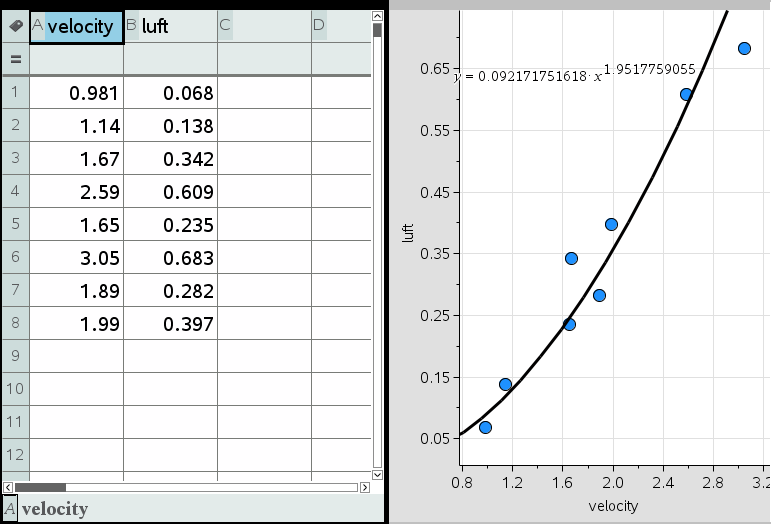
\includegraphics[width=\linewidth]{Ligningforluftmodstand.png}
\end{center}

\end{document}
